\documentclass[withindex, glossary]{cam-thesis}
\pdfminorversion=7

\usepackage[spanish]{babel}
\usepackage[utf8]{inputenc}
\usepackage[T1]{fontenc}
\usepackage[table]{xcolor}
\usepackage{multirow}
\usepackage{tabularx}
\usepackage{graphicx}
\usepackage{lmodern}
\usepackage{cleveref}

\usepackage{hyperref}
\addto\extrasspanish{%
    \def\chapterautorefname{capítulo}%
}

\usepackage{svg}
\usepackage{multicol}
\usepackage{mathtools}
\usepackage{booktabs}
\usepackage{bookmark}
\usepackage{blkarray, bigstrut}
%\usepackage{subcaption}
\usepackage{pgfgantt}
\usepackage{array}
\usepackage[capposition=top]{floatrow}

\usepackage[backend=biber, style=ieee, sorting=ynt]{biblatex}
\addbibresource{thesis.bib}

\usepackage{minted}
\usemintedstyle{manni}

\usepackage{csquotes}

\usepackage{tikz}
\usetikzlibrary{shapes.geometric, arrows.meta, fit, backgrounds, positioning, matrix, decorations.pathreplacing, calc}
\tikzstyle{startstop} = [rectangle, rounded corners, minimum width=3cm, minimum height=1cm,text centered, draw=black, fill=red!50]
\tikzstyle{io} = [trapezium, trapezium left angle=70, trapezium right angle=110, minimum width=3cm, minimum height=1cm, text centered, draw=black, fill=blue!30]
\tikzstyle{process} = [rectangle, minimum width=3cm, minimum height=1cm, text centered, draw=black, fill=orange!30]
\tikzstyle{decision} = [diamond, minimum width=3cm, minimum height=1cm, text centered, draw=black, fill=green!20]
\tikzstyle{database} = [cylinder, minimum width=3cm, minimum height=2cm, text centered, shape border rotate=90, aspect=0.25, draw=black, fill=yellow!30]
\tikzstyle{arrow} = [thick, ->, >=stealth]
\tikzstyle{line} = [-Latex]
\newcommand{\inline}[2]{%
    \begin{tikzpicture}[baseline=(word.base), txt/.style={shape=rectangle, inner sep=0pt}]
        \node[txt] (word) {\texttt{#1}};
        \node[above] at (word.north) {\footnotesize{#2}};
    \end{tikzpicture}%
}

\usepackage{pgfplots}
\pgfplotsset{compat=newest}

\setlength{\columnseprule}{0.4pt}

\title{Estudio sobre sistemas de anti-aliasing e implmenetación de anti-aliasing temporal}
\author{Hugo Ferrando Seage}
\college{U-Tad}
\submissiondate{septiembre 2018\\Tutor: Alberto Sánchez Campos}
\date{September 2018}
\fecha{septiembre 2018}

% PDF meta-info
\subjectline{Máster en Computación Gráfica y Simulación}
% max 6
\keywords{opengl antialiasing temporal}

% Abstract
\espabstract{%
    Debido a la resolución limitada de las pantallas al \gls{rasterizar} gráficos 3D se deforman ciertas lineas y curvas. Este fenómeno se llama aliasing. La demanda de gráficos cada vez más realistas ha propiciado la creación de diferentes técnicas y algoritmos para disimular estos defectos, sin tener que recurrir necesariemente a pantallas de mayor resolución.

    El antialiasing se ha vuelto una técnica crucial para mejorar la calidad de imagen en el software con gráficos tridimensionales. Este campo de la computación gráfica lleva años desarrollandose, con nuevas técnicas publicadas continuamente.

    Este proyecto tiene como objetivo el análisis de las distintas técnicas existentes en el estado del arte y la implementación de un algoritmo de temporal antialiasing, compatible con motores con deferred shading y comparable en calidad al multisampling, junto a otras propiedades.
}

\abstract{%
    When rasterizing 3D graphics using computer screens, due to their limited resolution some lines and curves will become deformed. This phenomena is called aliasing. The ever increasing demand for more realistic graphics has driven the creation of new techniques and algorithms to hide these artifacts, without necessarily using higher resolution screens.

    Antialiasing has become a crucial technique to advance image quality in graphics software. This field has been explored for years, with new approaches being developed continually.

    This projects aims to analyze different antialiasing techniques developed and the implementation of a temporal antialiasing technique, compatible with deferred shading engines and with similar quality to mutlisampling, amongst other benefits.
}

% Glossary
\newglossaryentry{rasterizar}{%
    name=rasterizar,
    description={Conversión de una imagen descrita con alguna primitiva (curvas, vectores, triangulos) a un conjunto de pixels}
}

\newglossaryentry{opengl}{%
    name=OpenGL,
    description={API estándar para el desarollo de software con gráficos 2D o 3D con aceleración por hardware\cite{Kessenich:2016:OPG:3013620}}
}

% Acronyms

% Contents
\begin{document}
\frontmatter{}

% Thesis body:
\chapter{Introducción}
\section{¿Qué es el aliasing?}

El antialiasing es la deformación de ciertos elementos gráficos al ser rasterizados y plasmados en una pantalla con una resolución finita\cite{Mitchell:1988:RFC:378456.378514}. Normalmente los bordes de la geometría que tengan ángulos que no se alineen perfectamente con los pixels presentaran bordes de sierra abruptos, que no es fiel a la escena como se vería de forma natural.

Este proyecto se centra en aliasing dentro del campo de la computación gráfica, pero afecta a otras disciplinas, como el procesamiento de señales (por ejemplo al digitalizar señales de audio analógicas). En general, al representar valores continuos en algún medio discreto siempre habrá algún defecto de este tipo\cite{Mitchell:1988:RFC:378456.378514}.

Existen otros tipos de aliasing, como en el interior de texturas o al mover la camera rápidamente.

\section{¿Qué es el antialiasing?}

El antialiasing es el conjunto de técnicas cuyo objetivo es el de disimular o eliminar estas imperfecciones.

\chapter{Planteamiento del problema}

\section{Aliasing en bordes de geometría}
imagen

\section{Aliasing de texturas}
Posibles soluciones: Mip Maps, LoD

\section{Specular Aliasing}
\section{Motion Aliasing}
Explicar motion blur en cámaras

Accumulation motion blur (ps2+)
Per pixel motion blur (ps3+)
Per object motion blur (ps3+)

\chapter{Objetivos}

Este proyecto tiene dos objetivos principales:

\begin{enumerate}
    \item Analizar el estado del arte en el campo de la computación gráfica en relación al anti-aliasing. Explorar los problemas que presenta el aliasing en gráficos 2D y 3D, la evolución de las soluciones y los desarrollos en curso.
    \item El segundo objetivo es el de integrar una solución de anti-aliasing temporal a un motor gráfico 3D existente desarrollado durante la asignatura de \"APIs tridimensionales\" del Máster en Computación Gráfica y Simulación cursado.
\end{enumerate}

\chapter{Estado del Arte}

\section{Filtrado}
\label{filtros}

En gráficos raster (bidimensionales) el anti-aliasing se realiza mediante filtros.Para entender el filtrado en imágenes es necesario pensar en pixels no como pequeños cuadrados en una pantalla, si no en muestras de una función (normalmente 3 muestras, una por cada canal RGB)\cite{Smith95apixel}. Los filtros (o kernels) transforman las funciones para intentar suavizar los cambios bruscos de color.

En la figura~\ref{gls} se muestra una comparación de las diferentes formas en las que cada filtro interpola valores de una imagen con un solo canal. Cada punto representa la muestra de la función que se visualizará en la pantalla.

%\cite{resampling}

\begin{figure}[!htb]
    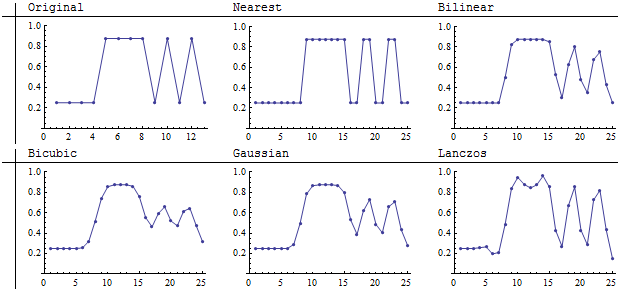
\includegraphics[width=\linewidth]{figures/Lw6ei.png}
    \caption{Comparación de interpolación usando diferentes filtros\cite{gis}}
    \label{gls}
\end{figure}

\begin{figure}[!htb]
    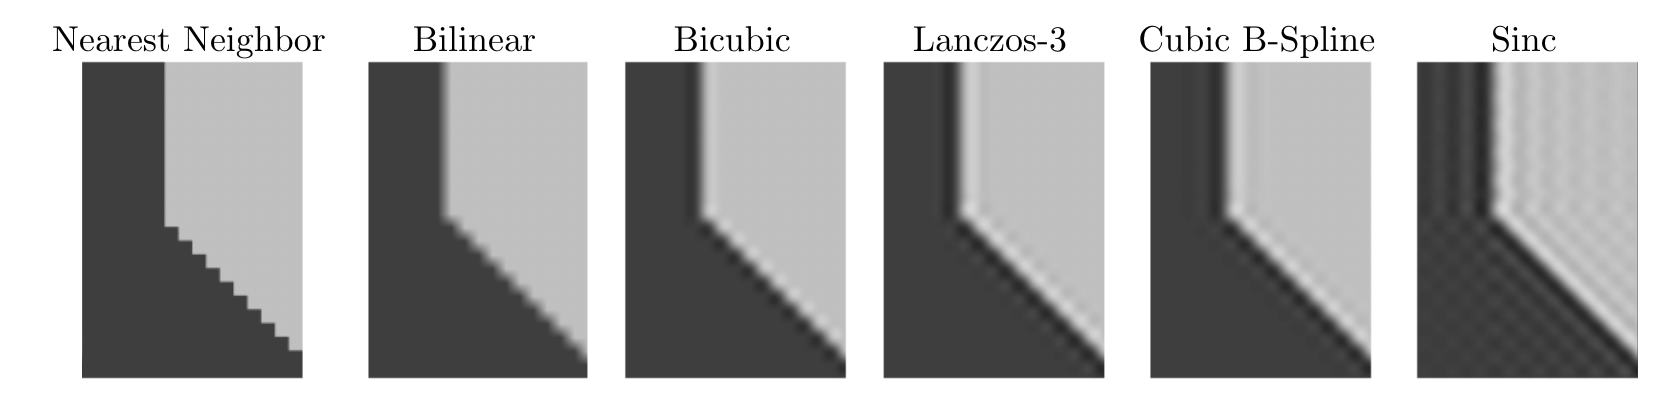
\includegraphics[width=\linewidth]{figures/comparison-filter.png}
    \caption{Comparación de resultados de diferentes filtros\cite{resampling2}}
\end{figure}

\section{Supersampling Antialiasing}

El supersampling consiste en minimizar el aliasing usando imágenes con una resolución mayor a la usada para su visualización (antialiasing espacial). Cada pixel en la pantalla será representado por más de un pixel en la imagen. Para el color final normalmente se hace la media del valor de los colores de los múltiples pixels.

Estas técnicas consumen más ancho de banda y memoria, ya que los buffers tienen que guardar más información por pixel que la imagen original.

La calidad del supersampling viene dado por la cantidad de samples por pixel y la técnica para saber que pixels usar en la imagen con mayor resolución para cada pixel de la pantalla.

En comparación a otras técnicas de antialiasing esta corrige aliasing de texturas y especular, además de aliasing de geometría. Esto se debe a que los subsamples los coge de en toda la escena.

%http://www.x86-secret.com/articles/divers/v5-6000/datasheets/FSAA.pdf

\subsection{Ordered Grid Supersampling}

En esta técnica de supersampling la distribución de los samples es uniforme. Debido a la naturaleza regular de este patrón, los subpixels se encuentran situados en forma de dos columnas y dos filas. Para lineas muy planas, tanto en horizontal como vertical el antialiasing no será muy efectivo, ya que muy rápidamente tocará dos subpixels en fila o columna y hasta el final no tocará los otros subpixels\ref{ogss}.

Este efecto se puede reducir usando más samples, pero el impacto en el rendimiento será todavía mayor.

Desde 2014 Nvidia ha publicado una técnica llamada Dynamic Super Resolution\cite{960}, que consiste en renderizar software a mayor resolución y usar OGSS con un filtro de blur gaussiano. En 2015 AMD implementó una técnica similar llamada Virtual Super Resolution.

\begin{figure}[!htb]
    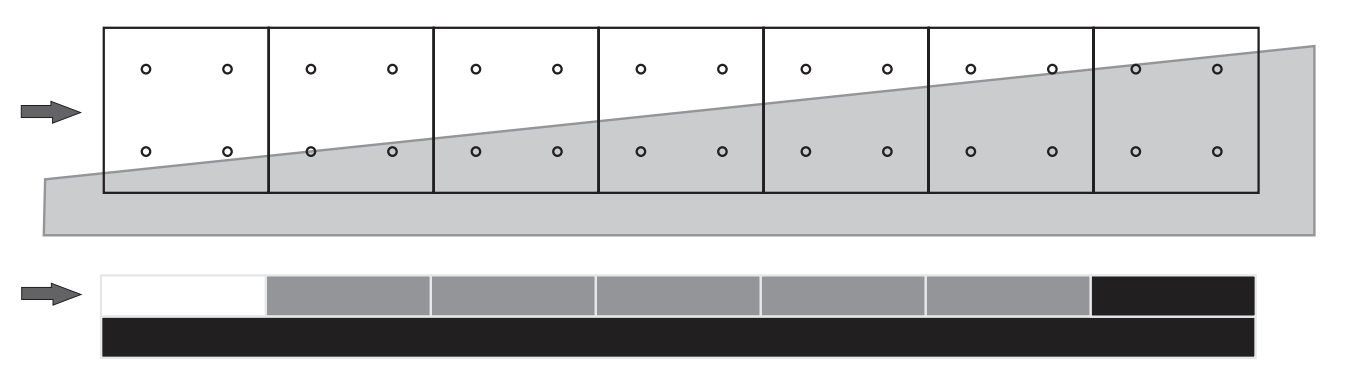
\includegraphics[width=\linewidth]{figures/ogss.png}
    \caption{Ordered Grid Super-Sampling\cite{Beets2000SupersamplingAA}}
    \label{ogss}
\end{figure}

\subsection{Rotated Grid Supersampling}

Aquí la idea es cambiar el lugar de los subsamples para minimizar la cantidad de columnas y filas. La distribución sigue siendo uniforme, pero el problema del aliasing en lineas muy planas se soluciona\ref{rgss} sin tener que recurrir a aumentar de manera significativa el numero de subsamples.

\begin{figure}[!htb]
    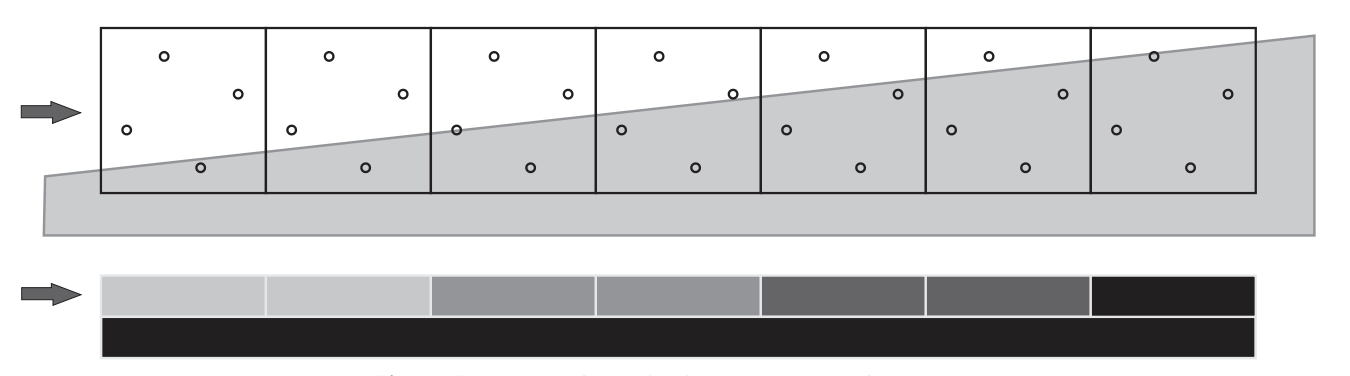
\includegraphics[width=\linewidth]{figures/rgss.png}
    \caption{Rotated Grid Super-Sampling\cite{Beets2000SupersamplingAA}}
    \label{rgss}
\end{figure}

\subsection{Quincunx Supersampling}

Este patrón es interesante como técnica de supersampling ya que usa subsamples localizados en las esquinas de los pixels, lo que permite reutilizar varios subsamples entre pixels\ref{fig:quincunx}. Esto permite una calidad similar a la de un antialiasing 4x pero con un coste computacional de un supersampling 2x. Aún así al reutilizar subsamples produce resultados algo más borrosos que otros métodos.

Aunque este patrón se pueda usar para supersampling Nvidia lo implementó en hardware desde la GeForce 3\cite{hraa} para acelerar el calculo de su multisampling. Sony al utilizar una GPU de Nvidia en la PS3 también disponía de esta tecnología en la consola.

\begin{figure}[!htb]
    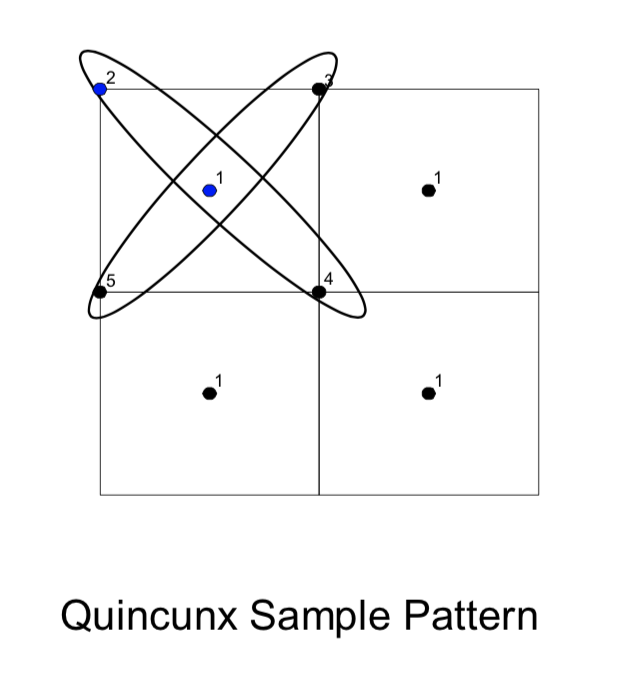
\includegraphics[width=\linewidth]{figures/quincunx.png}
    \caption{Quincunx Pattern\cite{hraa}}
    \label{fig:quincunx}
\end{figure}

\section{Multisampling}

Multisampling es una optimización del supersampling. Se sigue usando subpixels, pero en vez de resolver el color para cada subpixel el color se resuelve una única vez por pixel. Después de resolver el color se calcula el stencil buffer y depth buffer con subpixels, y dependiendo de la cantidad de subpixels que estén contenidos dentro del triangulo se usará un porcentaje del valor del color calculado. Esto reduce drásticamente el impacto en el rendimiento de la aplicación, ya que solo hay que acceder una vez por pixel a la textura, pero solo soluciona aliasing en los bordes de la geometría.

En el centro de un polígono todos los subpixels van a estar contenidos dentro, pero el color solo se calcula una vez (por ejemplo en el centro del pixel), por lo que se usará el 100\% del color, pero puede contener aliasing. En cambio, en los bordes, algún subpixel estará fuera de la geometría, por lo que se usará un porcentaje del color calculado, suavizando el borde.

Otra de las desventajas del multisampling anti-aliasing es que, tradicionalmente, no se puede usar en motores con deferred shading. Debido a que el calculo del color final de cada pixel se realiza en un pixel shader posterior al calculo del g-buffer, al hacer el resolve del mutisampling no esta lista toda la información necesaria. Desde OpenGL 3.2 y Direct3D 10.1 esto ha cambiado gracias al explicit multisampling\cite{textureMultisample}. La creación del g-buffer ahora se puede realizar usando texturas mltisampled y al calcular la luz se puede acceder a los subsamples mediante la función texelfetch. Si se realiza de esta forma hay que sacrificar la creación automática de mipmaps y filtrado de texturas, aunque siempre se pueden implementar manualmente en shaders. Aún así muchos desarrolladores han optado por usar post-processing antialiasing al usar deferred shading.

\section{Post Processing Antialiasing}

Este tipo de antialiasing ha ganado popularidad durante los últimos años, debido en parte al uso del deferred shading en los últimos motores gráficos. Los algoritmos presentados a continuación se pueden considerar filtros de rasters, como los de la sección\ref{filtros}, pero están pensados para ser usados en motores gráficos. Además, en muchos casos, usan información que no esta presente en la textura final, como pueden ser texturas de profundidad o vectores de movimiento,

\subsection{Fast Approximate Anti-aliasing}

El FXAA\cite{FXAA} es un sistema de anti-aliasing de post procesado desarrollado por NVIDIA\@.

\subsection{Morphological Antialiasing}
%https://software.intel.com/en-us/articles/morphological-antialiasing-mlaa-sample
mlaa

\subsubsection{Enhanced Subpixel Morphological Antialiasing}
%http://www.iryoku.com/smaa/downloads/SMAA-Enhanced-Subpixel-Morphological-Antialiasing.pdf
smaa

\subsection{Temporal Antialiasing}

El temporal antialiasing es un tipo de antialiasing de post procesado, pero que amortiza el coste computacional usando múltiples samples en múltiples frames. Esto presenta unas complicaciones a la hora de escoger samples en frames anteriores en imágenes no estáticas.

\chapter{Desarrollo}

Para este proyecto se ha integrado un sistema de anti-aliasing temporal en un motor de gráficos 3D que usa \Gls{opengl} como API gráfica.

\section{Jitter}

\section{Motion Vectors}

\section{Combinación de texturas}

\section{Neighborhood Clamping}

\section{Sharpening kernel}

\chapter{Resultados}

\begin{figure}[!htb]
    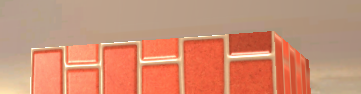
\includegraphics[width=\linewidth]{figures/taaoff.png}
    \caption{Anti-aliasing off}
\end{figure}

\begin{figure}[!htb]
    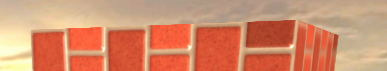
\includegraphics[width=\linewidth]{figures/taa8.png}
    \caption{Temporal anti-aliasing con 8 samples}
\end{figure}

\begin{figure}[!htb]
    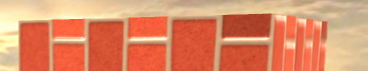
\includegraphics[width=\linewidth]{figures/taa16.png}
    \caption{Temporal anti-aliasing con 16 samples}
\end{figure}

\chapter{Conclusión}

% Bibliography:
\nocite{*}
\printbibliography{}

\listoffigures
\listoftables

% Index
\printthesisindex{}

\end{document}
